\documentclass{beamer}
\usetheme[faculty=med]{fibeamer}
\usepackage[utf8]{inputenc}
\usepackage[
  main=english
]{babel}        %% typeset as follows:
%% These macros specify information about the presentation
\title{Sistemas Operacionais} %% that will be typeset on the
\subtitle{Processos e threads} %% title page.
\author{Guilherme Meira}
%% These additional packages are used within the document:
\usepackage{ragged2e}  % `\justifying` text
\usepackage{booktabs}  % Tables
\usepackage{tabularx}
\usepackage{tikz}      % Diagrams
\usetikzlibrary{calc, shapes, backgrounds, positioning}
\usepackage{minted}
\usepackage{amsmath, amssymb}
\usepackage{url}       % `\url`s
\usepackage{listings}  % Code listings
\usepackage{xcolor}
\definecolor{highlightcolor}{RGB}{255, 140, 119}
\setminted{highlightcolor=highlightcolor}
\frenchspacing
\begin{document}
  \frame{\maketitle}
  \AtBeginSection[]{% Print an outline at the beginning of sections
  	\begin{frame}<beamer>
  		\frametitle{Agenda}
  		\tableofcontents[currentsection]
  	\end{frame}}
  	
\section{Processos}
\begin{frame}{Processos}
   	\begin{itemize}
   		\item \textbf{Processos} são o conceito mais central de qualquer sistema operacional
   		\item Um processo representa um \alert{programa em execução}
   		\item Processos permitem que um computador realize varias tarefas ao mesmo tempo, mesmo quando apenas uma CPU está disponível
   	\end{itemize}
   	\begin{figure}
   		
\includegraphics[width=0.3\paperwidth]{resources/multitask}
   	\end{figure}
\end{frame}
\begin{frame}{Processos}
	\begin{itemize}
		\item Computadores modernos estão sempre realizando diversas tarefas ao mesmo tempo:
		\begin{itemize}
			\item Navegando na web
			\item Tocando música
			\item Checando novos e-mails
			\item Buscando por vírus
			\item Copiando arquivos
			\item Dentre várias outras
		\end{itemize}
		\item O sistema operacional faz com que a CPU troque muito rapidamente entre processos, dando a impressão de que estão executando em paralelo (\textbf{pseudoparalelismo})
		\item Sistemas com vários processadores serão estudados mais adiante
	\end{itemize}
\end{frame}
\begin{frame}{Processos}
	\begin{itemize}
		\item Computadores modernos estão sempre realizando diversas tarefas ao mesmo tempo:
		\begin{itemize}
			\item Navegando na web
			\item Tocando música
			\item Checando novos e-mails
			\item Buscando por vírus
			\item Copiando arquivos
			\item Dentre várias outras
		\end{itemize}
		\item O sistema operacional faz com que a CPU troque muito rapidamente entre processos, dando a impressão de que estão executando em paralelo (\textbf{pseudoparalelismo})
		\item Sistemas com vários processadores serão estudados mais adiante
	\end{itemize}
\end{frame}
\begin{frame}{Processos}
	\begin{itemize}
		\item O \textbf{program counter (PC)} é um registrador da CPU que aponta para a posição de memória que contém a próxima instrução a ser executada
	\end{itemize}
	\begin{figure}
		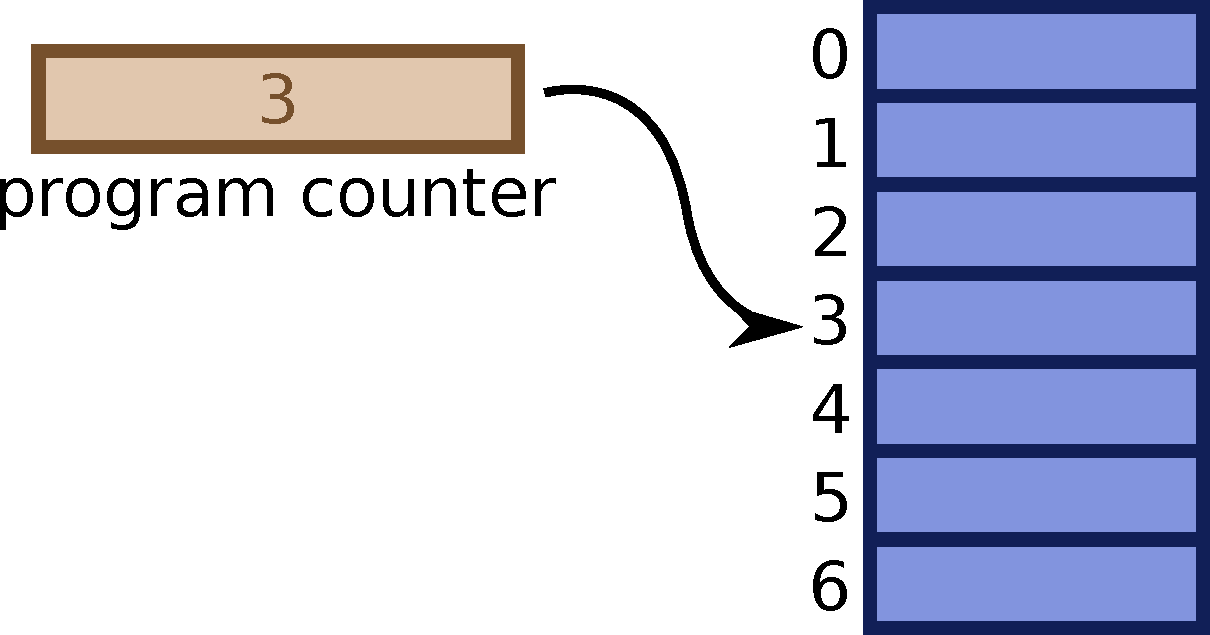
\includegraphics[width=0.5\paperwidth]{resources/pc}
	\end{figure}
\end{frame}
\begin{frame}{Processos}
	\begin{itemize}
		\item Uma CPU tem apenas um program counter
		\item O sistema operacional precisa armazenar o program counter de cada processo na memória
		\item Quando um processo vai receber um tempo da CPU, seu program counter é carregado no program counter real da CPU
	\end{itemize}
	\begin{figure}
		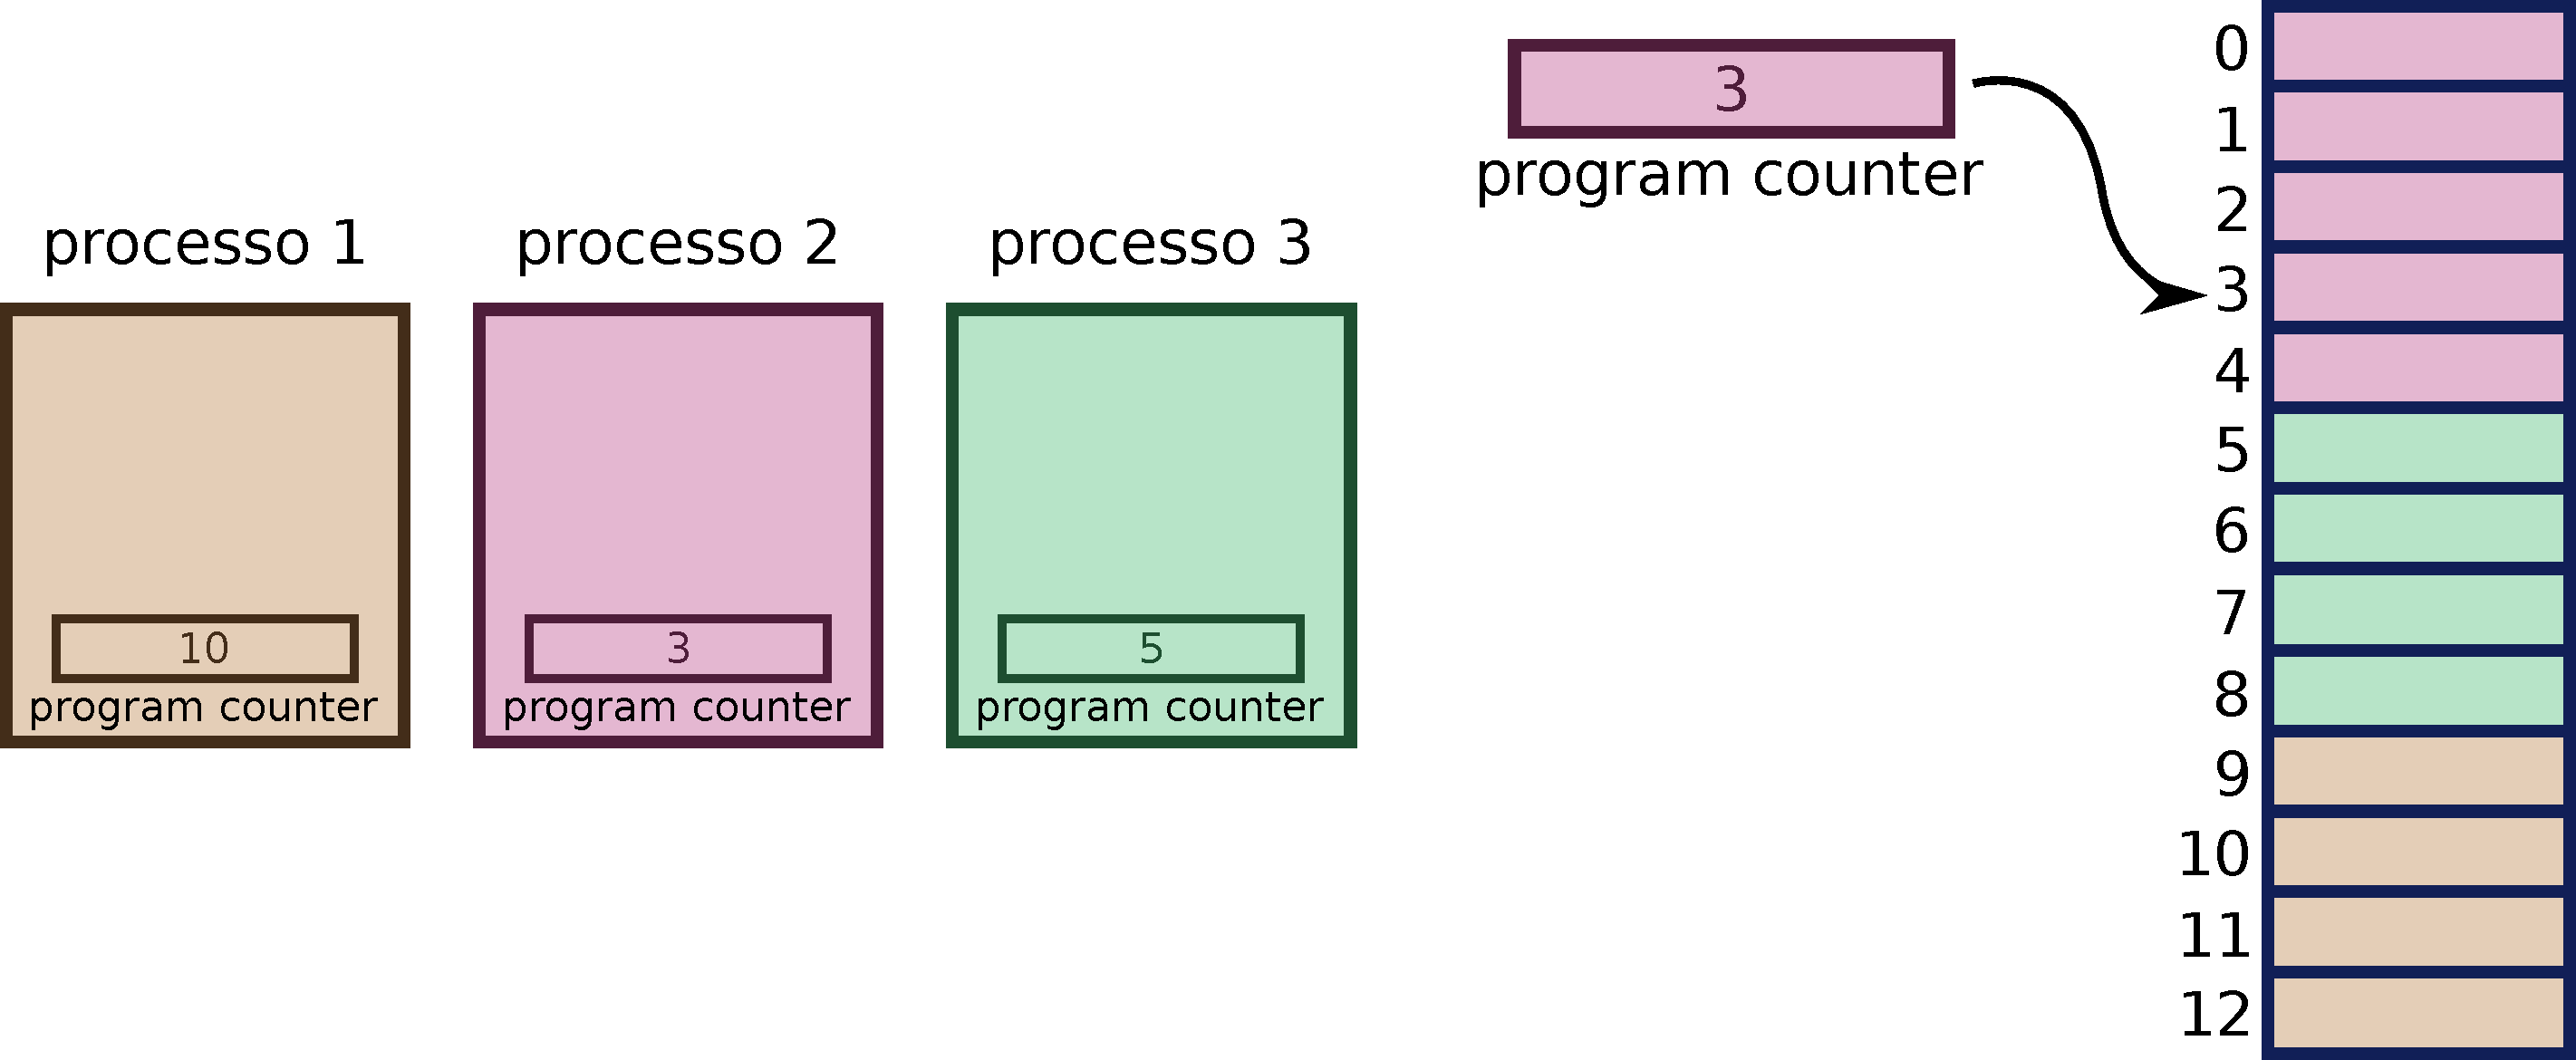
\includegraphics[width=0.8\paperwidth]{resources/pc2}
	\end{figure}
\end{frame}
\begin{frame}{Processos}
	\begin{itemize}
		\item O sistema operacional determina quando um processo vai executar e por quanto tempo ele vai ter a posse da CPU
		\item Para a maioria dos processos isso não é relevante
		\item Isso pode afetar processos com requerimentos de tempo real (ex: tocar áudio e video em sincronia)
	\end{itemize}
	\begin{figure}
		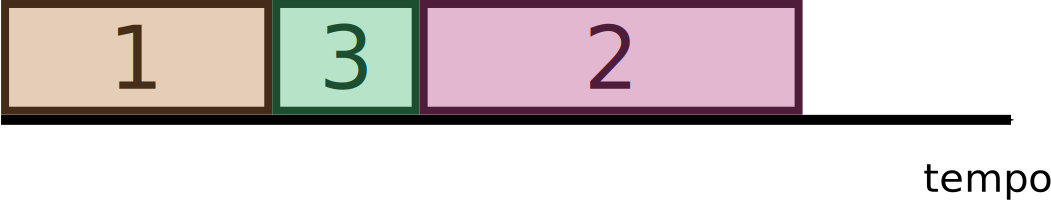
\includegraphics[width=0.5\paperwidth]{resources/time}
	\end{figure}
\end{frame}
\begin{frame}{Processos}
	\begin{itemize}
		\item Qual a diferença entre um \textbf{processo} e um \textbf{programa}? \pause
		\item Uma analogia:
		\begin{itemize}
			\item Uma pessoa está fazendo um bolo seguindo uma receita
			\item A pessoa é o \textbf{processador}, a receita é o \textbf{programa}, a ação de fazer o bolo é o \textbf{processo}
			\item A pessoao é interrompida pelo filho que foi picado por uma abelha
			\item Ele anota onde parou na receita e pega um livro de primeiros socorros para ajudar o filho
			\item Aqui, trocamos de um processo para o outro
			\item Quando ele termina de cuidar do filho, continua o processo anterior de onde parou
		\end{itemize}
	\end{itemize}
\end{frame}
\begin{frame}{Processos}
	\begin{itemize}
		\item Um \textbf{programa} é uma sequência de passos que pode ficar guardada em disco sem fazer nada
		\item Um \textbf{processo} é a atividade de executar as instruções de um programa
		\item O mesmo programa pode ser executado mais de uma vez ao mesmo tempo por processos diferentes
	\end{itemize}
\end{frame}
\begin{frame}{Processos}
	\framesubtitle{Criação de processos}
	\begin{itemize}
		\item Durante a execução de um sistema operacional, processos podem ser criados por diversos motivos:
		\begin{itemize}
			\item Inicialização do sistema
			\item Execução de uma chamada de sistema por um processo que já esteja rodando
			\item O usuário requisita a criação de um processo
			\item Inicio de um lote
		\end{itemize}
	\end{itemize}
\end{frame}
\begin{frame}{Processos}
	\framesubtitle{Criação de processos}
	\begin{itemize}
		\item Quando o sistema operacional é iniciado, vários processos são criados
		\item Alguns são processos de primeiro plano, que interagem com o usuário
		\item Outros rodam em segundo plano, e não estão associados a um usuário em específico, mas a uma tarefa
		\item Processos que ficam rodando em plano de fundo são chamados de \textbf{daemons}
	\end{itemize}
\end{frame}
\begin{frame}{Processos}
	\framesubtitle{Criação de processos}
	\begin{itemize}
		\item Em UNIX, processos são criados pela chamada de sistema \alert{\texttt{fork}}
		\item Essa chamada cria um clone do processo que a chamou
		\item O novo processo, então, pode executar a chamada \alert{\texttt{execve}} para carregar um novo programa
		\item No Windows, processos são criados pela chamada \alert{\texttt{CreateProcess}}
		\item Tanto em Windows como em UNIX, cada processo tem seu próprio espaço de endereçamento (não é possível acessar a memória de outro processo)
	\end{itemize}
\end{frame}
\begin{frame}{Processos}
	\framesubtitle{Término de processos}
	\begin{itemize}
		\item Após serem criados, processos eventualmente são terminados, por diversos motivos:
		\begin{itemize}
			\item Saída normal (voluntário)
			\item Saída com erro (voluntário)
			\item Erro fatal (involuntário)
			\item Morto por outro processo (involuntário)
		\end{itemize}
	\end{itemize}
\end{frame}
\begin{frame}{Processos}
	\framesubtitle{Hierarquia de processos}
	\begin{itemize}
		\item Em UNIX, processos possuem uma hierarquia
		\item Um processo e seus filhos formam um \textbf{grupo}. Quando o usuário envia um sinal a um processo, todos os processos do grupo recebem o sinal (veremos sinais com mais detalhes adiante)
		\item Quando o UNIX inicializa, um processo especial chamado \alert{\texttt{init}} cria todos os demais processos. O \texttt{init} é o pai de todos os processos no UNIX
		\item O Windows não possui o conceito de hierarquia de processos
	\end{itemize}
\end{frame}
\begin{frame}{Processos}
	\framesubtitle{Estados de um processo}
	\begin{itemize}
		\item Um processo pode estar em um de três estados:
		\begin{itemize}
			\item [Executando] o processo está utilizando a CPU no momento
			\item [Pronto] o processo está pronto para rodar, mas o sistema operacional não o deu a posse da CPU
			\item [Bloqueado] o processo está esperando algum evento externo para poder rodar
		\end{itemize}
	\end{itemize}
	\begin{figure}
		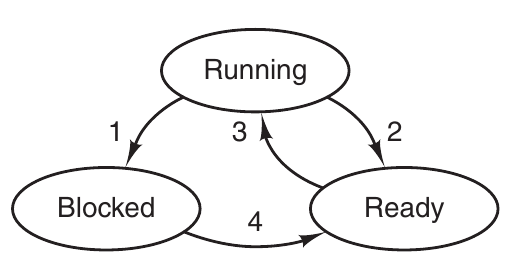
\includegraphics[width=0.5\paperwidth]{resources/states}
	\end{figure}
\end{frame}
\begin{frame}{Processos}
	\framesubtitle{Estados de um processo}
	\begin{itemize}
		\item As transições no diagrama representam:
		\begin{enumerate}
			\item Processo bloqueia para esperar por algum evento
			\item Escalonador do sistema escolhe outro processo para colocar na CPU
			\item Escalonador escolhe este processo
			\item O evento que estava sendo aguardado acontece
		\end{enumerate}
	\end{itemize}
	\begin{figure}
		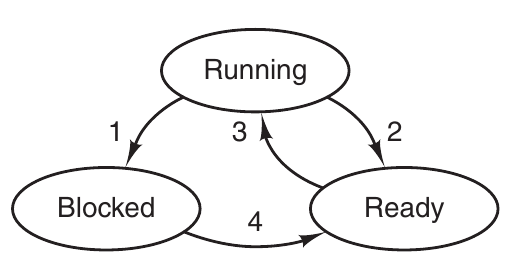
\includegraphics[width=0.5\paperwidth]{resources/states}
	\end{figure}
\end{frame}
\begin{frame}{Processos}
	\framesubtitle{Estados de um processo}
	\begin{itemize}
		\item O estado \textbf{bloqueado} é fundamentalmente diferente dos demais
		\item Enquanto nos estados \textbf{executando} e \textbf{pronto} o processo deseja ser executado, no estado \textbf{bloqueado}, mesmo com a CPU disponível o processo não pode rodar
		\item Um processo pode entrar nesse estado, por exemplo, para esperar uma entrada vinda do teclado ou de outro processo
		\item As transições entre os estados \textbf{executando} e \textbf{pronto} são geradas por uma parte do sistema operacional chamada de \alert{escalonador} (veremos mais detalhes adiante)
	\end{itemize}
\end{frame}
\begin{frame}{Processos}
	\framesubtitle{Implementação de processos}
	\begin{itemize}
		\item O sistema operacional mantém uma \alert{tabela de processos} contendo todas as informações sobre o estado do processo
		\item Essas informações são salvas quando o processo vai de \textbf{executando} para \textbf{pronto} ou \textbf{bloqueado} e são restauradas quando o processo for voltar a rodar
		\item As informações armazenadas na tabela de processos variam de sistema para sistema, mas em geral possuem informações sobre o próprio processo, sobre gerência de memória e sobre gerência de arquivos
	\end{itemize}
\end{frame}
\begin{frame}{Processos}
	\framesubtitle{Modelando multiprogramação}
	\begin{itemize}
		\item \textbf{Multiprogramação} é o uso da CPU por vários processos
		\item Ela permite que aumentemos a utilização da CPU
		\begin{itemize}
			\item Se um processo faz computação 20\% do tempo, 5 processos executando em multiprogramação manteriam a CPU ocupada 100\% do tempo
			\item Modelo pouco realista! Assume que os processos nunca estarão aguardando por I/O ao mesmo tempo
		\end{itemize}
	\end{itemize}
\end{frame}
\begin{frame}{Processos}
	\framesubtitle{Modelando multiprogramação}
	\begin{itemize}
		\item Podemos utilizar probabilidade para encontrarmos um modelo melhor:
		\begin{itemize}
			\item Um processo passa uma fração $p$ do tempo esperando por I/O
			\item Com $n$ processos na memória, a probabilidade de que todos os processos estejam esperando por I/O (isto é, a CPU está ociosa) é $p^{n}$
			\item A utilização da CPU é, então, calculada por:
			\begin{equation*}
			utilizacao_{CPU} = 1 - p^{n}
			\end{equation*}
		\end{itemize}
	\end{itemize}
\end{frame}
\begin{frame}{Processos}
	\framesubtitle{Modelando multiprogramação}
	\begin{itemize}
		\item Assim, podemos plotar a utilização estimada da CPU em função do número de processos em execução:
	\end{itemize}
	\begin{figure}
		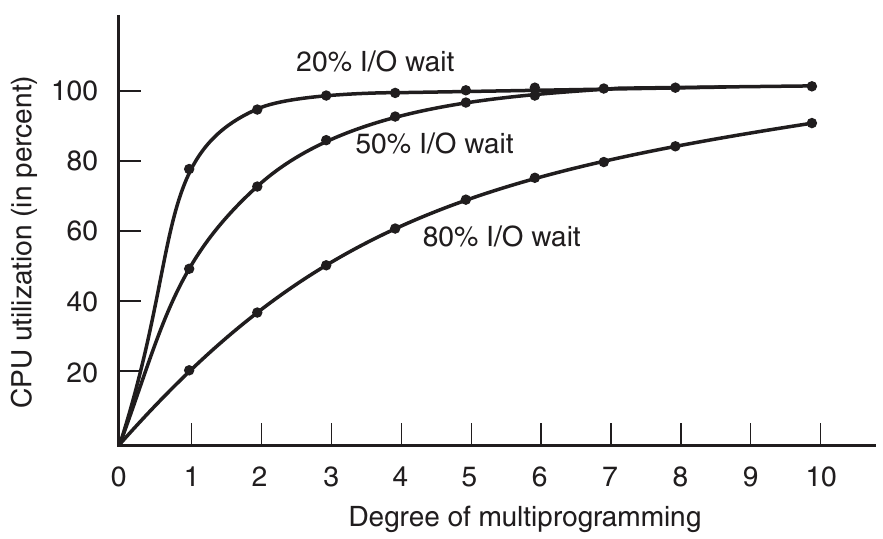
\includegraphics[width=0.7\paperwidth]{resources/multiprog}
	\end{figure}
 \end{frame}
 \begin{frame}{Processos}
 	\framesubtitle{Modelando multiprogramação}
 	\begin{itemize}
 		\item Este modelo também é uma aproximação, pois assume que os processos são independentes entre sí
 		\item Quando dois processos estão no estado \textbf{pronto}, apenas um pode utilizar a CPU e o outro terá que esperar, portanto, existe uma dependência entre os processos
 		\item Poderíamos chegar a modelos mais complexos utilizando Teoria das Filas, mas esse modelo é suficiente para fazermos algumas predições
 	\end{itemize}
 \end{frame}
 \begin{frame}{Processos}
  	\framesubtitle{Modelando multiprogramação}
  	Suponha que um computador tenha 8GB de memória. O sistema operacional ocupa 2GB e cada processo executando na máquina também ocupa 2GB.
  	\begin{itemize}
  		\item Quantos processos podem executar simultaneamente nesta máquina? \pause
  		\begin{itemize}
  			\item Três
  		\end{itemize}
  		\item Se o tempo de espera por I/O é de 80\%, qual é a utilização da CPU? \pause
  		\begin{itemize}
  			\item $1 - 0.8^{3} \approx 49\%$
  		\end{itemize}
  		\item Se adicionarmos mais 8GB de memória, qual será a nova utilização da CPU?
  		\begin{itemize}
  			\item Poderemos ter 7 processos em paralelo: $1-0.8^{7} \approx 79\%$
  		\end{itemize}
  	\end{itemize}
  \end{frame}
  \begin{frame}{Processos}
   	\framesubtitle{Modelando multiprogramação}
   	Ou seja, adicionar 8GB de memória aumentou a ocupação da CPU em 30\%. E se adicionássemos mais 8GB? \pause
   	\begin{itemize}
   		\item Podemos ter até 11 processos: $1 - 0.8^{11} \approx 91\%$
   		\item Ganhamos apenas mais 12\% de ocupação da CPU
   	\end{itemize}
\end{frame}
\section{Threads}
\begin{frame}{Threads}
	\framesubtitle{Modelando multiprogramação}
	Ou seja, adicionar 8GB de memória aumentou a ocupação da CPU em 30\%. E se adicionássemos mais 8GB? \pause
	\begin{itemize}
		\item Podemos ter até 11 processos: $1 - 0.8^{11} \approx 91\%$
		\item Ganhamos apenas mais 12\% de ocupação da CPU
	\end{itemize}
\end{frame}
\end{document}